\documentclass{beamer}
\usepackage{beamerthemesplit}
% \usepackage{pstricks}
\usepackage{graphicx}
\usepackage{mdwlist}
\usepackage{lineno, hyperref}

\usepackage{amssymb,latexsym,amsmath,amsthm,bbm}
\usepackage{hyperref}
\usepackage{tikz}
\usepackage[english]{babel}
\usepackage[latin1]{inputenc}
\usepackage{multirow}
\usepackage{verbatim}
\usepackage{alltt}
\usepackage{mycommands}

\usepackage{cmbright}
\renewcommand*\familydefault{\sfdefault}
\usepackage[T1]{fontenc}


\definecolor{wp-red}{RGB}{204,0,0}
\definecolor{wp-gray}{RGB}{51,51,51}
\definecolor{reynolds-red}{RGB}{153,0,0}
\definecolor{pyroman-flame}{RGB}{209,81,34}
\definecolor{hunt-yellow}{RGB}{253,215,38}
\definecolor{genomic-green}{RGB}{125,140,31}
\definecolor{innovation-blue}{RGB}{66,126,147}
\definecolor{bio-indigo}{RGB}{65,86,161}

\setbeamercolor{structure}{fg=wp-red}
\setbeamercolor{title}{bg=white, fg=wp-red}  % changes color on title page
\setbeamerfont{title}{series=\bfseries, size=\huge}
\setbeamerfont{author}{series=\bfseries, size=\Large}
\setbeamerfont{institute}{series=\mdseries, size=\large}

\setbeamercolor{frametitle}{bg=wp-red, fg=white}  % changes color at top of frame
\setbeamerfont{frametitle}{series=\bfseries}
\setbeamercolor{title in head/foot}{fg=white, bg=wp-red}  % changes color for title in footer
\setbeamerfont{title in head/foot}{series=\bfseries}
\setbeamercolor{author in head/foot}{fg=white,bg=wp-gray}  % changes color for author in footer
\setbeamerfont{author in head/foot}{series=\bfseries}


\title[Spatiotemporal Modeling of Extreme Events] % (optional, use only with long paper titles)
{
  Spatiotemporal Modeling of Extreme Events
}
\author[B. Reich and S. Morris]{Brian Reich and Samuel Morris}
\institute[NCSU]{North Carolina State University}
\date{}

\begin{document}

\begin{frame}\frametitle{\ }
\begin{center}
	\maketitle
\end{center}
\end{frame}

\begin{frame}{Motivation}
  \begin{itemize} \setlength{\itemsep}{1em}
    \item Average behavior is important to understand, but it does not paint the whole picture.
    \begin{itemize}
      \item e.g. When constructing river levees, engineers need to be able to estimate a 100-year or 1000-year flood levels.
    \end{itemize}
    \item In geostatistical analysis, kriging uses spatial correlation to help inform prediction at unknown locations.
    \item Want to explore ways to incorporate this spatial correlation when estimating the tails of the distribution.
  \end{itemize}
\end{frame}

\begin{frame}{Introduction to extremes}
  \begin{itemize} \setlength{\itemsep}{0.5em}
    \item Max-stable processes (Cooley et al., 2012):
    \begin{itemize}
      \item Consider a spatial process $x_t(\bs)$, $t = 1, \ldots, T$.
      \item Let $M_T(\bs) = \left\{ \bigvee_{t=1}^T x_t(\bs_1), \ldots, \bigvee_{t=1}^T x_t(\bs_n) \right\}$
      \item If there exists normalizing sequences $a_T(\bs)$ and $b_T(\bs)$ such
      that for all sites, $\bs_i, i = 1, \ldots, d$,
      \begin{align*}
        a_T^{-1}(\bs) \left\{ M_T(\bs) - b_T(\bs) \right\} \converged Y(\bs)
      \end{align*}
      which has a non-degenerate distribution, then $Y(\bs)$ is a max-stable process.
    \end{itemize}
  \end{itemize}
\end{frame}

\begin{frame}{General approaches}
  \begin{itemize}
    \item Two standard approaches:
    \begin{enumerate}[1.] \setlength{\itemsep}{0.5em}
      \item Block maxima:
      \begin{itemize}
        \item Uses yearly maxima
        \item Discards many observations
      \end{itemize}
      \item Peaks-over-threshold
      \begin{itemize}
        \item Incorporates more data than block maxima
        \item Autocorrelation may be an issue between observations (e.g. flood levels don't dissipate overnight)
      \end{itemize}
    \end{enumerate}
  \end{itemize}
\end{frame}

\begin{frame}{Univariate distribution functions}
  \begin{itemize}
    \item Generalized extreme value distribution (GEV):
    \begin{align*}
      \Pr(Y_j < y) = G_j(y) = \exp \left\{ -\left[ \left(1 + \xi_j \frac{y - \mu_j}{\sigma_j}\right)_+^{-1/\xi_j} \right] \right\}
    \end{align*}
    \item Generalized Pareto distribution (GPD):
    \begin{align*}
      \Pr(Y_j > y | Y_j > T) = F_j(y) = \left( 1 + \xi_j \frac{y - T}{\sigma_j} \right)_+^{-1/\xi_j}
    \end{align*}
  \end{itemize}
\end{frame}

\begin{frame}{Multivariate representations}
  \begin{itemize}
    \item Multivariate distributions:
    \begin{itemize}
      \item Assume common standardized max-stable marginal, like unit-Fr\'{e}chet
      \begin{align*}
        \Pr(Z < z) = exp(-z^{-1})
      \end{align*}
      \item The multivariate representation for the GEV is
      \begin{align*}
        \Pr(\bZ \le \bz)  &= G^*(\bz) = \exp(-V(\bz))\\
                V(\bs)    &= d \int_{\Delta_d} \bigvee_{i = 1}^d \frac{w_i}{z_i} H(\ddd w)
      \end{align*}
      where
      \begin{itemize}
        \item $\Delta_d = \{ \bw \in \calR^d_+ \mid w_1 + \cdots + w_d = 1\}$
        \item $H$ is a probability measure on $\Delta_d$
        \item $\int_{\Delta_d}w_i H(\ddd w) = 1 / d$ for $i = 1, \ldots, d$.
      \end{itemize}
    \end{itemize}
  \end{itemize}
\end{frame}

\begin{frame}{}
  \begin{itemize} \setlength{\itemsep}{0.5em}
    \item Although $V(\bs)$ can be flexible, the number of parameters is unwieldy.
    \begin{itemize}
      \item For an asymmetric logistic dependence, we have $2^d - d - 1$ free parameters
    \end{itemize}
    \item New model builds on existing geostatistical methods.
  \end{itemize}
\end{frame}

\begin{frame}{Skew-normal distribution}
  \begin{itemize} \setlength{\itemsep}{0.5em}
    \item Assume observed data $Y_t(\bs)$ come from a skew-normal (Zhang and El-Shaarawi, 2012)
    \begin{align*}
      Y_t(\bs) = X_t(\bs)\beta + \alpha z_t + v_t(\bs)
    \end{align*}
    where
    \begin{itemize} \setlength{\itemsep}{0.25em}
      \item $\alpha \in \calR$ controls the skew
      \item $z_t \iid N_{(0, \infty)}(0, \sigma^2_t)$ is a random effect
      \item $v_t(\bs) \sim \text{MVN}(0, \Sigma)$ where $\Sigma_t$ is a spatial covariance matrix with variance $\sigma^2_t$
    \end{itemize}
  \end{itemize}
\end{frame}

\begin{frame}{Skew-normal distribution}
  \begin{itemize} \setlength{\itemsep}{0.5em}
    \item By conditioning on $\alpha$ and $z_t$
    \begin{align*}
      Y_t(\bs) \mid \alpha, z_t \sim \text{MVN}(\mu_t(\bs), \Sigma_t)
    \end{align*}
    where $\mu_t(\bs) = X_t(\bs) \beta + \alpha z_t$
    \item When $\sigma_t^2 \iid \text{IG}(a, b)$, then this becomes a multivariate $t$-distribution
    after marginalizing over the $\sigma_t^2$ terms.
    \item Can use standard geostatistical methods to fit this model.
    \item Predictions can be made through kriging.
  \end{itemize}
\end{frame}

\begin{frame}{Random daily partition}
  \begin{itemize} \setlength{\itemsep}{0.5em}
    \item Consider a set of daily knots $\{w_{t1}, \ldots, w_{tK}\}$ that define a daily partition
    $\{P_{t1}, \ldots, P_{tK}\}$ such that
    \begin{align*}
      P_{tk} = \{s : k = \argmin_\ell|| \bs - w_{t\ell}|| \}
    \end{align*}
    \item For $\bs \in P_{tk}$, the model becomes
    \begin{itemize}
      \item $\mu_t(\bs) = X_t(\bs) \beta + \alpha z_{tk}$
      \item $\sigma^2_t = \sigma^2_{tk}$
    \end{itemize}
    \item After marginalizing over the $\sigma_{tk}^2$ terms, $Y_t(\bs)$ is a multivariate $t$-distribution
    within the partition.
  \end{itemize}
\end{frame}

\begin{frame}{Thresholding data}
  \begin{itemize} \setlength{\itemsep}{0.5em}
    \item Tails of the distribution should speak for themselves.
    \item We threshold the observed data at a suitably high threshold $T$.
    \item Observations below the threshold are imputed during MCMC.
  \end{itemize}
\end{frame}

\begin{frame}{MCMC details}
  \begin{itemize} \setlength{\itemsep}{0.5em}
    \item Three main steps:
    \begin{enumerate}[1.]
      \item Impute missing observations and data below $T$
      \item Update parameters with random walk Metropolis Hastings or Gibbs sampling
      \item Make spatial predictions
    \end{enumerate}
  \end{itemize}
\end{frame}

\begin{frame}{Data analysis}
  \begin{itemize} \setlength{\itemsep}{0.5em}
    \item Ozone analysis at 85 sites in NC, SC, and GA for 92 days
    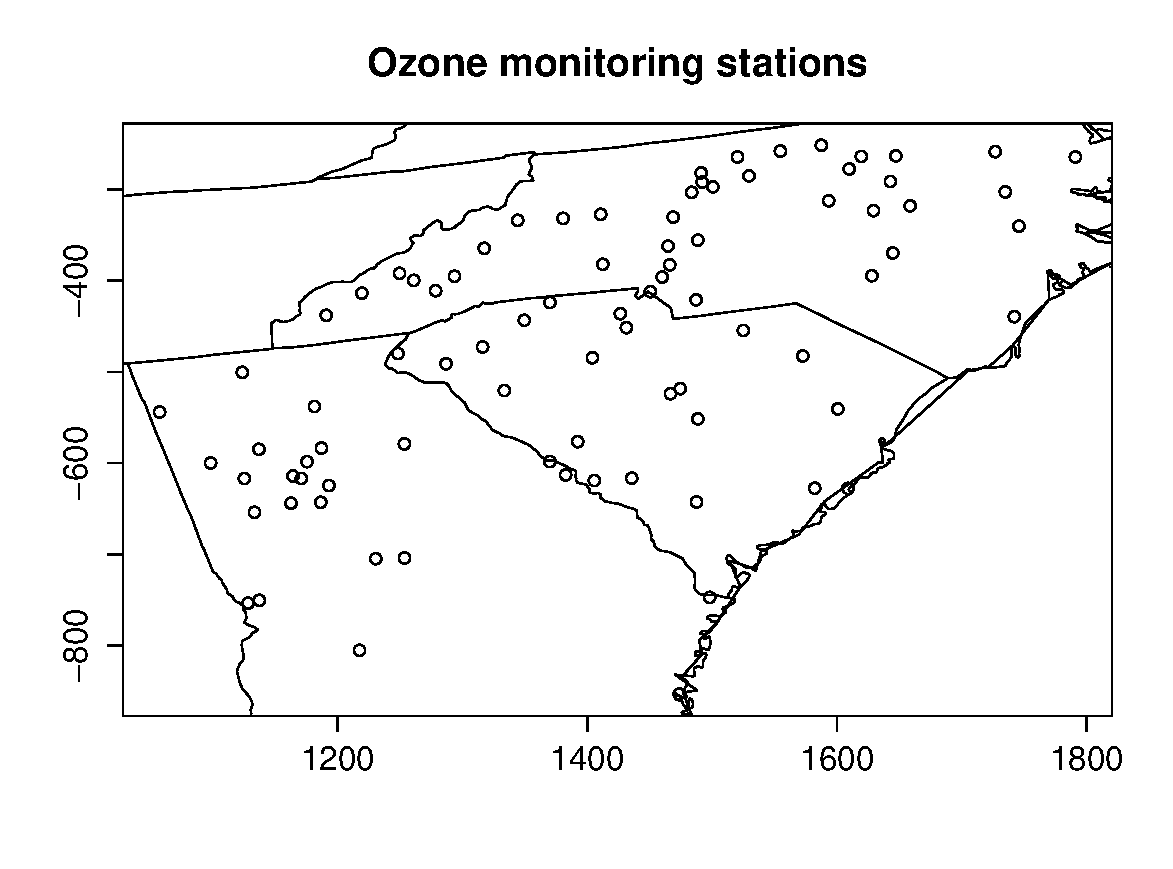
\includegraphics[width=1\linewidth]{./plots/ozone_station.pdf}
  \end{itemize}
\end{frame}

\begin{frame}{Model comparisons}
  \begin{itemize} \setlength{\itemsep}{0.5em}
    \item 9 different analysis methods
    \begin{enumerate}[1.]
      \item Gaussian
      \item $t$, $K=1$, $T=0$
      \item $t$, $K=5$, $T=0$
      \item $t$, $K=1$, $T=0.9$
      \item $t$, $K=5$, $T=0.9$
      \item skew-$t$, $K=1$, $T=0$
      \item skew-$t$, $K=1$, $T=0.9$
      \item skew-$t$, $K=5$, $T=0$
      \item skew-$t$, $K=5$, $T=0.9$
    \end{enumerate}
    \item Compare quantile scores using 5-fold cross validation
  \end{itemize}
\end{frame}


\begin{frame}{References}
  \begin{itemize} \setlength{\itemsep}{0.5em}
    \item Cooley, D., Cisewski, J., Erhardt, R. J., Mannshardt, E., Omolo, B. O. and Sun, Y. (2012) A survey of spatial extremes: Measuring spatial dependence and modeling spatial effects. {\it REVSTAT}, 10, 135--165.
    \item Zhang, H. and El-Shaarawi, A. (2010) On spatial skew-Gaussian processes and applications. {\it Environmetrics}, 33--47.
  \end{itemize}
\end{frame}

\end{document}